\documentclass[12pt]{article}

\usepackage[margin = .8in]{geometry}
\usepackage{amsmath}
\usepackage{graphicx}
\usepackage{multicol, enumerate, tabularx}

\usepackage{adjustbox}

\usepackage{fancyhdr}
\pagestyle{fancy}

\lhead{Math F113X: Numbers and Society}
\rhead{Date: \hspace{1in}}

\usepackage{tikz}
\usetikzlibrary{calc,trees,positioning,arrows,fit,shapes,through, backgrounds}
\usetikzlibrary{patterns}

\usetikzlibrary{decorations.markings}
\usetikzlibrary{arrows}

\usepackage{pgfplots}

\usepackage{longtable}
\usepackage{tabularx}

\newcommand{\ds}{\displaystyle}
\newcommand{\ans}[1][1in]{\rule{#1}{.5pt}}

\newcommand{\points}[1]{(#1 points.)}		% Trying to be lazy.

\usepackage{array}
\newcolumntype{L}[1]{>{\raggedright\let\newline\\\arraybackslash\hspace{0pt}}m{#1}}
\newcolumntype{C}[1]{>{\centering\let\newline\\\arraybackslash\hspace{0pt}}m{#1}}
\newcolumntype{R}[1]{>{\raggedleft\let\newline\\\arraybackslash\hspace{0pt}}m{#1}}
\newcommand{\red}[1]{\textcolor{red}{#1}}

\newcommand{\be}{\begin{enumerate}}
\newcommand{\ee}{\end{enumerate}}

%\topmargin -1in
%\textheight 9.5in
%\oddsidemargin -0.3in
%\evensidemargin \oddsidemargin
%\pagestyle{empty}
%%\marginparwidth 0.5in
%\textwidth 7in
%\parindent 0in

%--------------------------------------------------------------------------------------------------------------------------------------------------------------------------
%						Document
%--------------------------------------------------------------------------------------------------------------------------------------------------------------------------


\begin{document}
%\pagestyle{fancy}
\begin{center}
{\Large  Worksheet 15 (Scheduling 1): \\Priority Lists and Decreasing Time Algorithm}
\end{center}



\noindent \textbf{Group Names:} \hrulefill \\
%-------------------------------------------------------------------------------------------------------------
%						Assignment
%-----------------------------------------------------------------------------------------------------
\begin{enumerate}

\item The following tasks need to be completed for a project.

    \begin{tabular}{|c|c|c|}
      \hline
      {\bf Task} & {\bf Time Required} & {\bf Prerequisites} \\
      \hline
      A & 3 hours &  \\
      \hline
      B & 2 hours & \\
      \hline
      C & 1 hour & \\
      \hline
      D & 2 hours & A, B \\
      \hline
      E & 2 hours & A, B \\
      \hline
      F & 8 hours & C \\
      \hline
      G & 1 hours & D, E, F \\
      \hline
    \end{tabular}
  \be
  \item
 To the left of the chart, draw a digraph to represent this project.
 %   \vfill
    \item If there is only one processor, how long will it take to complete the project? \ans
    
    \item The critical time can be determined by looking at the longest sequence of tasks in the
digraph, called the critical path. 

What is the critical path for this project? \hrulefill 

What is the critical time? \ans
   
%   \vspace{1cm} 
\ee
\item Consider the following digraph:

\newcommand{\mydigraph}{\begin{tikzpicture}[vtx/.style={draw, circle, inner sep = 3pt, font = \scriptsize}, myto/.style={-latex, shorten >=2pt, shorten <=2pt
}, node distance = \r cm]
\node[vtx, label=above:{\scriptsize $T_{1}(10)$}, ] (T1) at (0,0){};
\node[vtx, right =of T1, label=above:{\scriptsize $T_{2}(7)$}] (T2) {};
\node[vtx, right =of T2, label=above:{\scriptsize $T_{3}(4)$}] (T3) {};
\node[vtx, below = \s cm of T1, label=above:{\scriptsize $T_{4}(9)$}] (T4) {};
\node[vtx, right =of T4, label=above left:{\scriptsize $T_{5}(5)$}] (T5) {};
\node[vtx, right =of T5, label= right:{\scriptsize $T_{6}(4)$}] (T6) {};
\node[vtx, below =\s cm of T4, label=below:{\scriptsize $T_{7}(13)$}] (T7) {};
\node[vtx, right =of T7, label=below:{\scriptsize $T_{8}(4)$}] (T8) {};
\node[vtx, right =of T8, label=below:{\scriptsize $T_{9}(6)$}] (T9) {};

\foreach \i/\j in {1/2,2/3,4/5,5/6,7/8,8/9,2/6,5/3,7/5,4/8}{\draw[myto] (T\i) -- (T\j);}
\end{tikzpicture}
}

\def\r{2}
\def\s{.6}
%\begin{center}
\begin{adjustbox}{valign=t,minipage={.4\textwidth}}
\mydigraph
\end{adjustbox}
%\end{center}
%\hspace{1cm}
\begin{adjustbox}{valign=t,minipage={.4\textwidth}}
\begin{tabular}{c | c | c}
time & ready & done \\ \hline
&&\\&&\\&&\\&&\\&&\\&&\\&&\\
\end{tabular}
\end{adjustbox}


\be
\item Create a schedule using the priority list 
\[T_{1}, T_{2}, T_{3}, T_{4}, T_{5}, T_{6}, T_{7}, T_{8}, T_{9}\]
assuming you have only two processors.

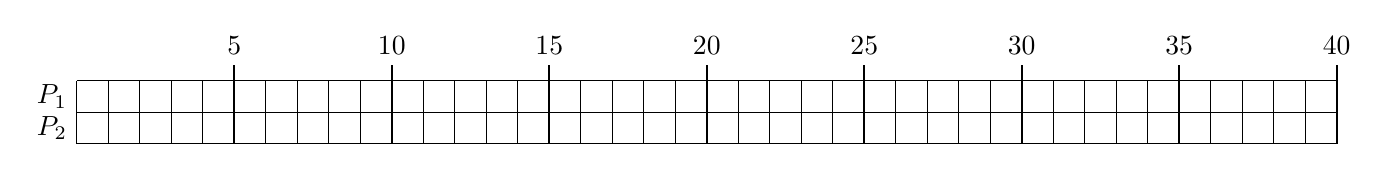
\begin{tikzpicture}[scale = .8]
\path (0, 3/4) node[left] {$P_{1}$};
\path (0, 1/4) node[left] {$P_{2}$};
\draw[step=1/2] (0,0) grid (40/2, 2/2);
\foreach \i in {5, 10, ..., 40}{\draw[thick] (\i/2,0) -- (\i/2,2/2+1/4) node[above]{\i};}
\end{tikzpicture}

\item How much idle time does processor 1 have? \ans 

How much idle time does processor 2 have? \ans

\newpage

\item Here's the digraph again. Create a schedule using the same priority list \[T_{1}, T_{2}, T_{3}, T_{4}, T_{5}, T_{6}, T_{7}, T_{8}, T_{9}\] assuming you have three processors.


%\begin{center}
\begin{adjustbox}{valign=t,minipage={.4\textwidth}}
\mydigraph
\end{adjustbox}
%\end{center}
%\hspace{1cm}
\begin{adjustbox}{valign=t,minipage={.4\textwidth}}
\begin{tabular}{c | c | c}
time & ready & done \\ \hline
&&\\&&\\&&\\&&\\&&\\&&\\&&\\&&\\
\end{tabular}
\end{adjustbox}

%\item Create a schedule using the same priority list \[T_{1}, T_{2}, T_{3}, T_{4}, T_{5}, T_{6}, T_{7}, T_{8}, T_{9}\] assuming you have three processors.

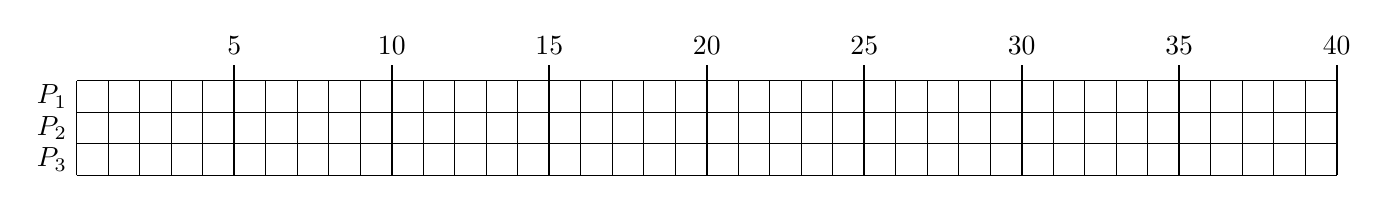
\begin{tikzpicture}[scale = .8]
\path (0, 5/4) node[left] {$P_{1}$};
\path (0, 3/4) node[left] {$P_{2}$};
\path (0, 1/4) node[left] {$P_{3}$};
\draw[step=1/2] (0,0) grid (40/2, 3/2);
\foreach \i in {5, 10, ..., 40}{\draw[thick] (\i/2,0) -- (\i/2,3/2+1/4) node[above]{\i};}
\end{tikzpicture}

\item How does the time to completion compare with using two processors?

\vspace{.5cm}

How does the idle time compare? \vspace{.5cm}

\item What is the critical path for this digraph? \hrulefill

Have you found an optimal schedule? How do you know?

\vspace{1cm}

\item The Decreasing Time Algorithm says: Create the priority list by listing the tasks in order from longest completion time to shortest completion time.


%\begin{center}
\begin{adjustbox}{valign=t,minipage={.4\textwidth}}
\mydigraph
\end{adjustbox}
%\end{center}
%\hspace{1cm}
\begin{adjustbox}{valign=t,minipage={.4\textwidth}}
\begin{tabular}{c | c | c}
time & ready & done \\ \hline
&&\\&&\\&&\\&&\\&&\\&&\\&&\\
\end{tabular}
\end{adjustbox}



 What priority list do you get if you prioritize the tasks using the Decreasing Time Algorithm?

\hrulefill

\item  Create a schedule using the priority list you just found using the Decreasing Time Algorithm,
assuming you have only two processors. How long does it take? \ans

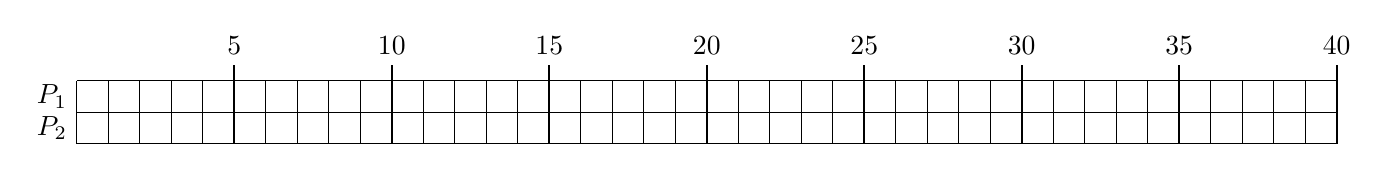
\begin{tikzpicture}[scale = .8]
\path (0, 3/4) node[left] {$P_{1}$};
\path (0, 1/4) node[left] {$P_{2}$};
\draw[step=1/2] (0,0) grid (40/2, 2/2);
\foreach \i in {5, 10, ..., 40}{\draw[thick] (\i/2,0) -- (\i/2,2/2+1/4) node[above]{\i};}
\end{tikzpicture}

How does it compare to your previous schedule?


\ee

%\item Go back to the original digraph you constructed in Problem 1. 
%\be
%\item What prioritization do you get if you use the Decreasing Time Algorithm for this list of tasks?
%
%\hrulefill
%
%\item What schedule do you get with that prioritization, using two processors?
%
%\begin{tikzpicture}[scale = .8]
%\path (0, 3/2) node[left] {$P_{1}$};
%\path (0, 1/2) node[left] {$P_{2}$};
%\draw[step=1] (0,0) grid (20, 2);
%\foreach \i in {5, 10, ..., 20}{\draw[thick] (\i,0) -- (\i,2+1/4) node[above]{\i};}
%\end{tikzpicture}
%\ee
%

\end{enumerate}
\end{document}

%-------------------------------------------------------------------------------------------------------------------------------------------------------------------------------------------------------------------

%%% Local Variables:
%%% mode: latex
%%% TeX-master: t
%%% End:
